\chapter{Methodology}
\label{methodology}

The methodology in this work describes all the considerations and steps taken to build a solution to the problem analyzed from the case study. As such, the methodology has a very close relationship with the case study. The problem studied addresses a situation where a person stores sensitive data on the cloud, with the intention of accessing and modifying such data at a later time. The solution itself is an \emph{implementation of a client-server based software} that makes use of a library called HElib, which enables the use homomorphic encryption on integers.

Even though the object of study is the application of homomorphic encryption in the cloud, it is not trivial to find a fitting situation where it can be applied. The search becomes more complex as the limitations of state-of-the-art homomorphic encryption tools are considered. For example, it is thought of a case study that is simple enough so that the currently available tools can be used effectively, and complex enough so that applying homomorphic encryption is compelling and better-suited than other alternatives.

This section discusses the case study and the means to offer a solution based on the cloud.  Then, it describes a proof of concept in a general way as a stand-alone solution. The tasks required for the proof of concept to work are briefly described, and some considerations regarding key management are noted. Afterwards, it mentions the scenario where a client-server architecture is employed, discussing some decisions that were made regarding the communication between the client and the server. Finally, it mentions how the aforementioned tasks are being split between each component.

\section{{Case Study}}

The case study considered for this work is explained as follows: commonly, a household has more than one member, e.g.\ partner and children. The responsible \emph{householders} (i.e.\ the parents) might want to keep an eye on the house while being away, especially if their children are left behind. They would like to ensure that their children stay inside during this time, and that nobody else, except for a babysitter, enters the house. And if it were the case that somebody got in or out, they would probably desire to be promptly notified of it. This holds true especially when they are away for long periods of time, during a vacation, for example. A traditional solution consists in setting up a surveillance system throughout the house, which would certainly work to prevent robbery, but wouldn't necessarily work as a measure to know whether or not the children have left the house. Additionally, such a system usually requires a montly or yearly fee. Therefore, setting up a surveillance system might be too costly for some families, and not be quite adaptive to their needs. It might be more effective to deploy a system that detects when people enter and exit the building through the main doors, and keep a counter of it. 

The main idea is that the \emph{surveillance counter} initializes at some point in time, and, as people go in and out, the counter increases or decreases, respectively. Setting up the sensors and other pieces of hardware can be considered as a Do-It-Yourself project, as resources could easily be found. Wilson \cite{wilson2005simultaneous} mentions several considerations to take when tracking people inside a building using binary sensors. In this case, however, it is simpler to set it up, as it is not necessary to keep track of the people inside the building: only if they go in or out past the main doors. 

The issue comes out when the recorded data, that is, the counter, is to be accessed or modified securely over the web. 

\section{{Proposed Solution}}

The proposed solution addresses the issue hinted at the end of the case study description. The counter data that is recorded by the sensors is to be sent to a server somewhere in the cloud, where it will be stored indefinitely, awaiting for the data to be accessed or modified in the future. It might not be appropriate to have a dedicated server at home for this functionality, which is why the computing task is instead delegated to the cloud. The data stored in the cloud server can be accessed from anywhere else; however, one of the most important aspects of the whole scheme remains unaddressed: confidentiality.

Usually, the householder would not allow others to know about the actual counter, including the cloud server itself, as this information is considered to be \emph{sensitive}. The traditional approach is to make use of public-key cryptography to \emph{encrypt} the data and prevent from anybody else to know the counter. Once the counter data has been encrypted successfully, it can then be safely uploaded to the server in the cloud. Then, when the householder desires to view the value of the counter, he would have to download the data and \emph{decrypt} it in order to view it. This sounds reasonable until changes are applied to this value, since it would have to go again through the encryption process. Indeed, this would imply that every time there is a change in the counter, the whole ciphertext would have to be reuploaded to the server. Considering that a person comes in and out of a building quite frequently, it would turn out to be a heavy burden that carries an overhead cost, computational and bandwidth-wise, that keeps accumulating every time there is an update. 

An alternative approach is to simply notify the cloud service of any changes that occur, so that it performs the addition or subtraction itself instead of relying on receiving the whole encrypted result. Even though this would not be possible to do with traditional cryptography, it can be done using \emph{homomorphic cryptography}. The concept behind this approach is that, while the initial counter value is being stored on the server, the client part that resides on the household sends over any change of individuals that come in our outside the building. Thus, the cloud service performs the appropriate homomorphic computations on the currently stored value. This occurs without the need of reuploading the counter data, as the cloud service has no need of decrypting the data in the first place. Since the full ciphertext is not being re-sent, the overhead costs are reduced significantly.

Whenever the householder needs to know the value of the counter, he can authenticate with the cloud service to download the current ciphertext that represents the counter. The ciphertext can be decrypted using the private key generated at the beginning of the process. This aspect remains the same whether homomorphic encryption is used or not, and there is no way around it without compromising confidentiality. Considering that a system that detects when people come in and out might not be perfect, and if somehow the counter gets to an incorrect value, it could be reset to the correct amount by the user as required. In this case, it would be unavoidable to send a newly encrypted counter value.

The solution itself consists in an implementation of a client-server software that aims to store and modify securely a counter by making use of homomorphic encryption. The various tasks that help reach this goal are distributed by the client and server components of the software. The client focuses on the initialization of the homomorphic encryption scheme, generation of public and private keys, encryption of initial counter data, among other things. On the other hand, the server is dedicated to store and manage the public key of the household and its current counter value. Both parts of the software utilize a library called HElib, which makes it possible to run homomorphic evaluations. In other words, this library is used to perform basic operations on the data, such as addition, subtraction, and multiplication. Consequently, it is also used to generate the public and private keys, encrypt data, and decrypt it. Once the encrypted counter is stored in the server, a different kind of client, i.e.\ the householder, can then ask to download and decrypt it. It makes sense to say that it will be a different kind of client, since most likely the interested person would not be at the household, i.e., place where the counter was initialized.

\section{{Details of the HElib library}}

An implementation of a homomorphic encryption scheme, the Brakerski-Gentry-Vaikuntanathan (BGV), is openly available as a C++ library, called HElib. Using this library, it is possible to encrypt integer values and perform operations on them while being encrypted. There are many parameters to be considered when using this implementation, and these usually define how the public and private keys are going to be like. For this particular application, most parameters can be left in their default values, as they seem to serve the intended purpose. 

Part of the description found in the code repository of HElib states that the library is considered to be low-level, and given its difficulty and constant changes, it is not that appropriate to build big applications with it. Regarding the use of the library and its implementation of homomorphic encrypted, often referred to as \emph{HE}, the following is stated: ``At its present state, this library is mostly meant for researchers working on HE and its uses. Also currently it is fairly low-level, and is best thought of as \emph{assembly language for HE}. That is, it provides low-level routines (set, add, multiply, shift, etc.), with as much access to optimizations as we can give.'' Brakerski et al.\ \cite{helib}.

It is important to note that the library recently started to support multi-threading, which would considerably speed up the evaluation times of the homomorphic operations. Not too long ago it started to support bootstrapping as well, a technique that prevents the ciphertext from getting too much noise and that eventually results in the incorrect homomorphic evaluations.

\section{Setting up the Parameters and Context}

The HElib library is an implementation of a homomorphic encryption scheme, and as such, it has certain requirements before it can encrypt data or even generate keys. First of all, it has a list of parameters which must be manually set. Depending on the parameters applied, some aspects that directly affect the keys and ciphertext are altered. The suggested values are used for the majority of the parameters. Altering the values of the parameters could be an interesting way to do experimentation with the key size and computation time required.

Table \ref{tbl:parameters} briefly describes each parameter used in HElib. It does not go into much depth, as those details are mostly pertaining to the algorithms in the library.

\begin{table}[h]
  \caption{Parameters used in HElib}
  \label{tbl:parameters}
\centering
  \begin{tabular}{|l|l|l|}
    \hline
    \textbf{Parameter} & \textbf{Description} & \textbf{Value} \\ \hline
    R  &     number of rounds &  default=1     \\ \hline
    p  &     plaintext base  & default=2  \\ \hline
    r  &     lifting  & default=1  \\ \hline
    d  &     degree of the field extension  & default=1  \\ \hline
    c  &     number of columns in the key-switching matrices  & default=2  \\ \hline
    k  &     security parameter & default=80  \\ \hline
    L  &     number of levels in the modulus chain  & default=heuristic  \\ \hline
    s  &     minimum number of slots  & default=0  \\ \hline
    repeat &  number of times to repeat the test & default=1  \\ \hline
    m   &    use specified value as modulus & optional  \\ \hline
    mvec &   use product of the integers as  modulus & optional \\ \hline
    gens &   use specified vector of generators & optional \\ \hline
    ords  &  use specified vector of orders & optional \\ \hline
  \end{tabular}
\end{table}


\section{{Key Generation and Serialization}}

As the scheme implemented in HElib is based on public-key cryptography, it requires the use of public and private keys. The owner of the data has to generate his own set of keys as the first step, and it is only the public key which he should be willing to share. The user then shares his public key with the cloud service by some means of registration, so he does not have to share it every time he makes use of the service. The public key is used to encrypt the counter data for the first time before sending it over to the server, and the server itself requires this public key in order to perform any homomorphic operation.
The generation of the keys is pseudorandom, so extra care should be taken as to not use a predictable seed, so that the public and private keys are not recreated by another party. 

In order to generate a set of keys, a component called a \emph{context} needs to be instantiated using certain parameters. Firstly, the public key is obtained by simply instantiating an object of the class \textit{FHESecKey}. Then, a copy of the public key is made as the foundation for the private key. This exact copy applies a method called \textit{GenSecKey(w)}, which takes \textit{w} as a seed to create the real private key. Finally, it goes through a process that computes key-switching matrices, which are used in the internal algorithms of the library to create the secret key. The code for these actions are shown below:

\begin{lstlisting}[caption={Key generation},label={lst:keyGeneration},numbers=left,escapeinside={@}{@}]
  FHEcontext* context;
  FHESecKey* secretKey;
  FHEPubKey* publicKey;  
  context = new FHEcontext(m, p, r);
  // Set of keys are initialized
  publicKey = new FHESecKey(*context);
  secretKey = publicKey;
  // Secret key is fully created by using these two methods
  secretKey->GenSecKey(w); 
  addSome1DMatrices(*secretKey); 
\end{lstlisting}

Before proceeding to encrypt the data, it is important to have the public key serialized and ready to send it to the server. Serialization is a popular term used to describe the encoding of objects and the objects reachable from them, into a string of bytes. Serialization is a term introduced by Oracle \cite{oracleserial}, and it is commonly used for lightweight persistence and communication via sockets. In this case, it is used as the means of temporarily storing the public key in a stream of bytes so it can be shared with a remote server that will be able to read such stream. Only after the contents of the saved object have been fully read, it will be possible to reconstruct the public key. Fortunately, the HElib provides a very simple way to do serialization, since the class \textit{FHESecKey} supports the $\ll$ operator which works quite nicely with a couple popular serialization classes in C++ called \textit{istringstream} and \textit{ostringstream}. The use of this class is showed as follows: 

\begin{lstlisting}[caption={Key serialization},label={lst:serializeKey},numbers=left,escapeinside={@}{@}]
  ostringstream pkstream;
  pkstream << *publicKey;
\end{lstlisting}

As shown in Code Snippet \ref{lst:serializeKey}, the data stored inside the public key object has been stored as a stream of bytes in a highly portable object from the \textit{ostringstream} class. Using this newly populated object, the public key can be shared using sockets.

\section{{Encryption of the Counter Value}}

In order the protect the value of the counter from being known from other parties, including the server itself, it must be encrypted. This means that an encryption algorithm, provided by the HElib, is to be used on the plaintext that represents the counter. The result of this process is a \emph{ciphertext}, which, unless provided with the corresponding private key, cannot be deciphered back to its plaintext form. 

Following the conventions defined in the HElib, objects from the \textit{EncryptedArray} and \textit{PlaintextArray} are initialized using the \textit{context} and \textit{G} as parameters which were previously set. \textit{PlaintextArray} can be seen as a container for the plaintext, whereas \textit{EncryptedArray} is seen as a general container that works as an medium between the plaintext and ciphertext data. Once it has been done, a method called \textit{encode} of the same class can be used on the PlaintextArray object to prepare the data for encryption. The ciphertext is stored in a different kind of container, which comes from the class \textit{Ctxt}. This container is initialized using the public key as argument. Afterwards, the encryption of the plaintext data can be done using a method of the \textit{EncryptedArray} object simply called \textit{encrypt}. This method receives as arguments the objects of the plaintext and ciphertext containers, and the public key. Therefore, even though \textit{PlaintextArray} and \textit{Ctxt} are containers for either the plaintext or ciphertext, respectively, the \textit{EncryptedArray} is the medium that supports the translatation from one to the other.

\begin{lstlisting}[caption={Encryption of the counter value},label={lst:encrypt},numbers=left,escapeinside={@}{@}]
  EncryptedArray ea(*context, G);
  PlaintextArray counter(ea);  
  counter.encode(people);
  Ctxt& encryptedCounter = *(new Ctxt(*publicKey));  
  ea.encrypt(encryptedCounter, *publicKey, counter); 
\end{lstlisting}

The ciphertext obtained from Code Snippet \ref{lst:encrypt} can be used in several ways: its value can be modified by adding, substracting or multiplying it by some arbitrary value, it could also be decrypted at any time using the private key, or it could be serialized as it was done with the public key, so another party, e.g.\ the server, can receive and store it.

\section{{Operation Flow: Single Component}}

Before attempting to break down the whole implementation in two parts for both the server and client, a proof of concept is implemented which combines the tasks of both parts into a single program. The flow of this program represents how the data gets transformed through several tasks. 

\begin{enumerate}
	\item Parameters to use with the HElib are arbitrarily chosen, while other required values are computed.
	\item Context of the HElib library is set.	
	\item Public and private keys are created using the context.
	\item Optionally, public key can be serialized into a file so it can be used later.
	\item The structures to store plaintext and ciphertext are declared.
	\item The initial counter value is set into the plaintext structure.
	\item The plaintext is encrypted using the public key and stored into the ciphertext structure.
	\item Values are arbitrarily added or substracted from the ciphertext.
	\item Ciphertext is decrypted using the private key, and its value is stored in another plaintext structure.
	\item Newly decrypted plaintext is printed to verify correct result from operations.
\end{enumerate}

\section{{Software Architecture and Data transmission}}

Even though the case study started out considering cloud services, an actual implementation of the application can be addressed with a client-server architecture. The client-server architecture is a popular model that consists of a two parts: a client and a server. Usually, the server just waits for any kind of request from a client to do some kind of task. Meanwhile, the client usually starts some kind of task, but depends on a response from the server to complete. Most of the time, the client depends on the server because it might have something that the client does not, like a database.

In this case, the implementation of the counter application is approached using a client-server model. The server represents the cloud service that stores, serves, and modifies the encrypted data on request, while the client plays the part of obtaining and encrypting the sensitive data. The client also takes care of tasks such as initializing the components defined by the library, generating the public and private keys, encrypting the data, and serializing the encrypted counter before sending it over to the server. Meanwhile, the server takes care of establishing the communication details via TCP sockets, reconstructing the received ciphertext, and performing operations on it. Although a more secure implementation would consider using the Secure Socket Layer (SSL), it is simplified to cover only the details pertaining the use of homomorphic encryption.

Once the user obtains the initial data, i.e.\ by counting the number of people currently in the house at a given time, he proceeds to feed the data to the client program, so it is encrypted using the public key. After the counter data has been encrypted successfully, the data is then sent to the server via sockets. There are two possible protocols that can be used for this part: UDP and TCP. UDP stands for User Datagram Protocol and is used in conjunction with the Internet Protocol. UDP works best when the data units that are being sent are very small. It is also a little bit problematic considering that it does not reassemble data packets once they have arrived at the destination. The other option that was considered was TCP, which stands for Transmission Control Protocol. It is a little friendlier to use in the sense that it reassembles datagrams in the correct order once they arrive at their destination. However, it adds a little bit of overhead cost since it adds a header section per segment. For this scenario, it is preferred to use TCP instead of UDP, especially since it might become complicated to keep track of the order that the data packets arrive.

\section{{Sending and Reading Serialized Data}}

The serialized data that is sent through sockets is sufficiently large so that the operation cannot be done with a single function call, which is why a few considerations have to be made in the implementation. It is recommended to have some kind of supporting function that continuously is attempting to send data to the server, until there are no bytes left.

The following snippet of code shows how the ciphertext is serialized using the \textit{ostringstream} class, and then a function call is made to a supporting function which continuously attempts to send all the remaining bytes to the server. It is relatively simple to keep track of how many bytes are being sent and how many are left, which is why it stops sending data when there are no bytes left.
% \n could cause problems later on...
\begin{lstlisting}[caption={Sending ciphertext to the server},label={lst:write},numbers=left,escapeinside={@}{@}]
  // Ciphertext is serialized
  ostringstream oss;
  oss << encryptedCounter;
  
  // Sends data to server unless there is an error
  if(sendalldata(sockfd, oss.str().c_str(), 
    &msgsize) == -1) {
      printf("ERROR. Only \%d bytes sent! \n", 
        msgsize);
  }

int sendalldata(int s, char const* buffer,  int *len)
{
  int total = 0; // bytes sent
  int bytesleft = *len; // bytes left to send
  int n;
  
  // Sends data until no more bytes are left
  while(total < *len) {
    n = send(s, buffer+total, bytesleft, 0);
    if (n == -1) { break; }
    total += n;
    bytesleft -= n;
  }
  *len = total; 
  if(n == -1) 
    return -1;
  else 
    return 0;
}
\end{lstlisting}

As it cannot be expected that the serialized ciphertext of great size will be succesfully sent with a single send function call, the same goes for the receiving end. Certain measures have to be taken so that all the data is received completely and in the appropriate order.

The following piece of code extracted from the server side where the ciphertext is being received. First of all, a buffer is declared and initialized with the size of the ciphertext, which was previously received. A function called \textit{bzero()} is used to prepare and empty the buffer. Then, a \textit{while} loop is done as long as there are bytes remaining to be received. As more iterations go by, more data is appended to the buffer. A couple of variables are used to keep in check how many bytes have been read and how many are still pending to be read.

\begin{lstlisting}[caption={Reading data from the client},label={lst:read},numbers=left,escapeinside={@}{@}]
  // Initializes buffer where the ciphertext is put into
  char* responseBuffer = new char[responseBufferSize];
  bzero(responseBuffer, responseBufferSize);
  bytes_read = 0;
  int bytes_remaining = responseBufferSize;
  int this_recv;
  // Keeps receiving data via recv()  as long as there are bytes missing
  while(bytes_remaining > 0) {    
    this_recv = recv(newsockfd, responseBuffer+bytes_read,
                bytes_remaining, 0); 
    if(this_recv <=0) error("error on receive");
    else {
      bytes_remaining -= this_recv;
      bytes_read += this_recv;
    }
  }
\end{lstlisting}

\section{{Reconstructing the Ciphertext}}

It was observed in Code Snippet \ref{lst:keyGeneration}  and Code Snippet \ref{lst:write} that serialization enabled persistence of the public key and ciphertext and made it easier for the object data to be sent via sockets. However, the serialized objects cannot be used the way they are received. In this case, the ciphertext was serialized before being sent to the server, and once it is properly received, the data must be used to reconstruct the original ciphertext object.
If this is not done, there is no way to perform operations on the ciphertext, or even decrypt it to know its value.

The following piece of code describes the steps to be taken in order to reconstruct the object that will contain the ciphertext. First of all, the buffer that was previously filled with data is copied into a string variable, then it goes through a couple of steps so it can be used as a \textit{istringstream} object. The preparation seems complicated, but the reconstruction of the ciphertext object is actually quite simple. Since HElib is friendly with the \textgreater\textgreater operators, it can be done in one step. This operator basically takes the data from one variable and puts it in another kind of variable, one being a \textit{istringstream} object, and the other a \textit{Ctxt} object.

\begin{lstlisting}[caption={Reconstruction of the ciphertext},label={lst:reconstruct},numbers=left,escapeinside={@}{@}]
  // Buffer that will hold the ciphertext is defined with the exact size
  string strBuffer((const char*) responseBuffer, bytes_read);
  istringstream serialCipher;
  serialCipher.str(strBuffer);

  // Copies buffer into the Ctxt object
  Ctxt receivedCipher(publicKey);
  serialCipher >> receivedCipher;
\end{lstlisting}

As it is observed in Code Snippet \ref{lst:reconstruct}, in order for the server to perform any kind of computation it requires both the ciphertext and its respective public key. That is why it is recommended to perform some kind of registration at the beginning, so that it is not necessary to share the public key every time a change is to be done on the ciphertext. 

\section{{Changes in the Counter}}

Once the initial value of the counter is received by the server, there are two possible scenarios that could occur next: the value gets viewed by the householder, or a change in the counter occurs. Whenever a significant change is observed by the client program, the change is promptly notified to the server, which could be either imply that the value goes up or down. When the cloud service receives the value of change, it either adds or subtracts it from the previously stored value. The change can then be known to the user by retrieving the encrypted counter.

\begin{lstlisting}[caption={Addition on the ciphertext},label={lst:addition},numbers=left,escapeinside={@}{@}]
  // Object for plaintext is initialized using the encrypted array object
  PlaintextArray ptxtChange(*ea);
  ptxtChange.encode(change); 
  // change is assumed to be an integer
  Ctxt ctxtChange(*publicKey); 
  // ciphertext object is defined 
  ea->encrypt(ctxtChange, *publicKey, ptxtChange);

  // addition is performed on counter value and change value
  encryptedCounter += ctxtChange;
\end{lstlisting}

Code Snippet \ref{lst:addition} focuses on performing addition on the original counter value; it only requires that the respective public key is present to do the proper initializations. Prior to performing the addition, it is assumed that the value that represents the change on the counter has been previously received and validated. The operation itself is quite simply, since it uses the common addition operator. 

As it has been mentioned, whenever a homomorphic evaluation is performed on the ciphertext, a small amount of noise is added to it, and after a certain threshold, the ciphertext becomes unusable, in the sense that it no longer decrypts back to the correct value. \emph{Bootstrapping} is an advanced technique in fully homomorphic encryption which allows more homomorphic evaluations to be run on a ciphertext. As an alternative to bootstrapping, however, it is possible to reset the counter, i.e.\ upload a newly created ciphertext with an initial counter value, so that more homomorphic evaluations can be performed on it.  Considering that the operations that will be done most of the time are addition and subtraction, this is not something that will occur often, but eventually will. As of December 2014, HElib includes bootstrapping as an optimization of the scheme, which would increase the number of operations that can be done on a ciphertext before the accumulated noise makes it impossible to decipher the encrypted value. However, as the implementation of this counter system was started before December 2014, it was not considered to make use of bootstrapping.

\section{{Operation Flow: Client and Server}}

The proof of concept that makes use of homomorphic encryption ends up being completely linear in the sense that it has no communication at all with different parts of the outside world. The case study implies that there is a set location where the counter is initialized and uploaded to the cloud, and a variable location where the value of it is accessed. Therefore, the proof of concept is translated into a client-server architecture, where the tasks are delegated accordingly. 

In Figure \ref{fig:clientserver}, a breakdown of the client-model architecture employed is depicted. As previously mentioned, the solution is split into two parts: client and server sides. Each side has specific tasks that must be performed independently. The figure was conceived as an attempt to organize the software structure and assign a functionality to one of the components. The client side is in charge of the tasks that are performed at the place where the counter is initialized, i.e.\ the household. Such tasks include: setting up the parameters and context required by the HElib, generating the set of public and private keys, registering the public key, encrypting the initial counter value, serializing the ciphertext, recording changes in the counter value, and decrypting the received ciphertext. The following illustration depicts the client-server architecture that was conceived. 

\begin{figure}[H]
  \centering 
  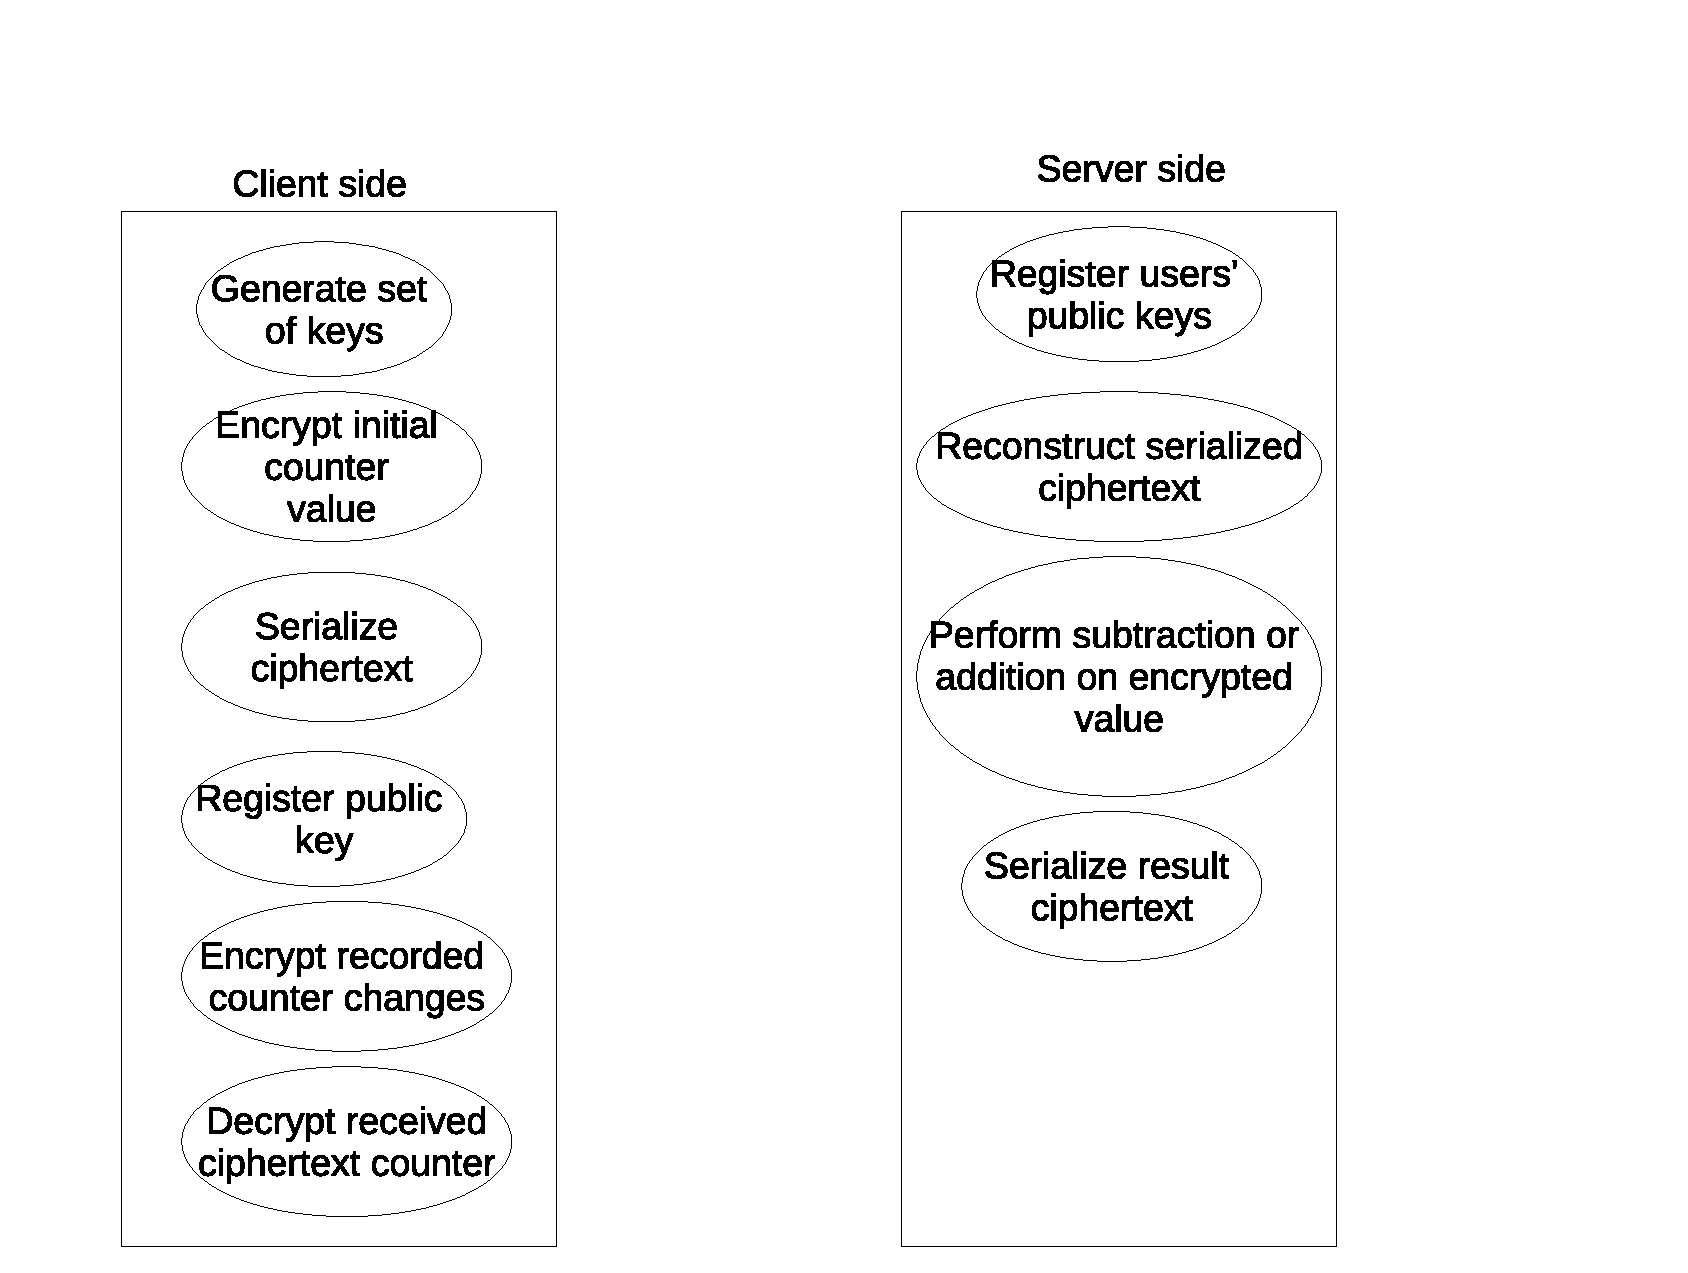
\includegraphics[scale=0.5]{clientserver}
  \caption{Architecture breakdown into client and server.}
  \label{fig:clientserver}
\end{figure}


In order to understand how the workflow occurs inside of the client-server architecture, it is better to think of two possible clients: one that is located at the household, and another one that requests access to the counter data. The sensor system is the former one, whereas the user is the latter. Usually, the client that retrieves data from the sensor begins by generating a set of keys and registering it with the server, and then encrypting the value of the initial counter before sending it over. Whenever a change of the value is notified to the server, it performs the corresponding operations: addition if people go inside, or subtraction if people go outside the building. Finally, whenever the user wants to learn the value of the counter, it can request to download it from the server. It is also possible for the user to reset the value of the counter as he sees fit. This flow of operation is shown in Figure \ref{fig:seqdiag} as a sequence diagram.

\begin{figure}[H]
  \centering
  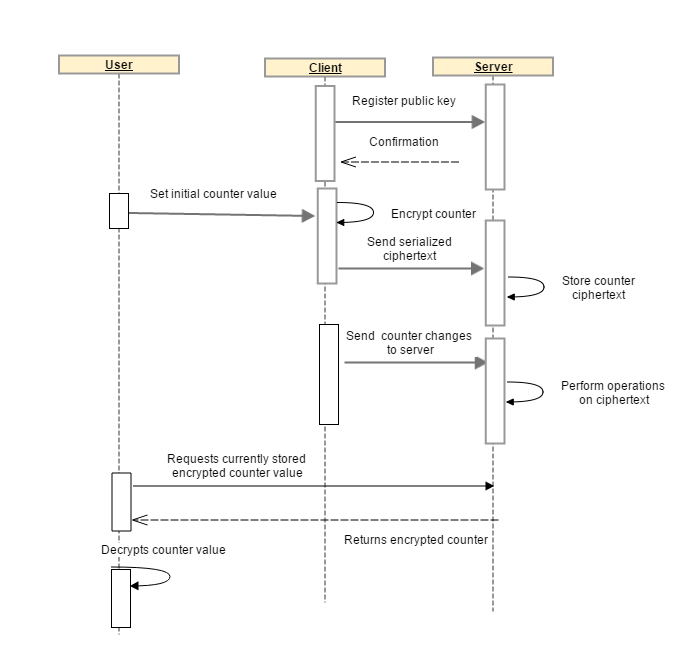
\includegraphics[scale=0.65]{counter}
  \caption{Sequence diagram showing operation under normal conditions}
  \label{fig:seqdiag}
\end{figure}

\section{Discussion}

The aspect of user registration is not part of the planned implementation itself, but it is recommended to consider how to handle different users. There might many more than a couple of households that make use of such a counting service. This is why each resident would have to register his public key and go through some kind of authentication mechanism every time they restart or download the counter data. It is especially important to take the appropriate measures so that somebody else does not reset the counter value of a household that is not theirs, because it would be chaotic when the resident looks at the counter and finds a value that does not represent reality.
To keep the registration under control, it might be ideal to keep a list of registered users either on a database or on a simple file for each household which would contain basic pieces of information such as an email address or username, along with the hash value of a password and the appropriate public key for the household that is being registered.

There were several problems at this stage that were directly related to the implementation. The transmission of serialized data between the client and server was especially problematic. The early attempts at sending serialized data to the server were not quite successful. Many different kind of errors were found, and the most common one was related to memory allocation. After going through several trial and error attempts, it was found the errors started appearing as the message got larger. This seemed to be inevitable as the default settings of a TCP blocking socket were not adequate to send large pieces of data. 

After doing the right adjustments, the problem seemed to go away, except that \textit{the result was not quite as expected}. It was known inmediately that something was up with the received ciphertext, as it could not decrypt properly. It helped to look at the data that the server received, and it was quite evident that it was not complete. Indeed, only certain fragments of the ciphertext were received successfully, which led to an incorrect decryption. Several adjustments were made to the process of receiving data, so that a couple of control variables were used to keep in check how many bytes were being received. It was set so that it would only stop reading data from the client until all of the bytes had been read and assembled in a buffer. Both the functionalities of reading and writing the ciphertext on a socket were relatively more complicated considering that it was done without the support of a framework that specialized on it.

%[TALK ABOUT DECRYPTION]
%(1 month later)->I forgot what i was going to say about decryption anyways

In summary, a description of the case study was given, a solution based on homomorphic encryption was proposed to tackle the problem found in the case study, details of the HElib were discussed, and all of the relevant considerations pertaining to the implementation were explained. These considerations took on points such as the parameters and context, key generation and serialization, software architecture, transmission of serialized data, reconstruction of the ciphertext, and applying changes to the counter. Finally, all of these tasks were addressed when considering a client-server implementation.

\clearpage
